%!TEX root = main.tex
\section{Discussion\label{sec:guidelines}}
% In this section, we first describe a model to help characterize the design space for VQS based on the analytical workload and usage patterns from different use cases. Then, we present design challenges related to each of the process.
\subsection{Characterizing Design Space for VQSs}
Visual querying often consists of searching for a desired visualization instance across a visualization collection (Z) for a fixed visualization axes (X,Y). To characterize the design space of VQS, we introduce two axes depicting the amount of information known about visualized attribute and pattern instance, as shown in Figure~\ref{2dmodel}.
\begin{figure}[h!]
  \centering
  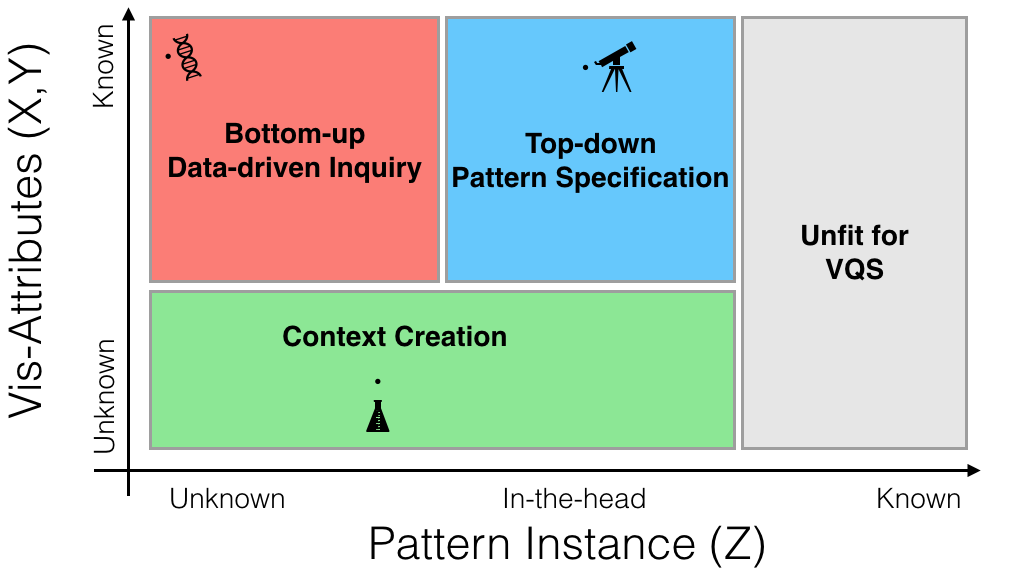
\includegraphics[width=\linewidth]{figures/2dmodel.png}
  \caption{The design space of VQSs is characterized by how much the analyst knows about the visualized attributes and pattern instance. Colored areas highlights the three different paradigms of VQSs.}
  \label{2dmodel}
\end{figure}
\par Along the \textbf{pattern instance} axis, the visualization instance may already be \texttt{known} to the analyst, exist as a pattern \texttt{in-the-head} of the analyst, or completely \texttt{unknown} to the analyst. For example, if a user wants to study only the pattern related to a specific gene, then the use cases is more suited for a visualization-at-a-time system, since the analyst can directly work with the visualization instance without the need for performing visual querying (Figure~\ref{2dmodel} grey). Most past VQSs assume that the analyst has a desired pattern in-the-head that could be conveyed through visual specification, such as a sketch. Inspired by Pirolli and Card's information foraging framework~\cite{Pirolli}, which distinguishes between information processing tasks that are \textit{top-down} (from theory to data) and \textit{bottom-up} (from data to theory), we define this process as ``top-down pattern specification'' (Figure~\ref{2dmodel} blue). On the other hand, in the realm of ``bottom-up data-driven inquiry'' (Figure~\ref{2dmodel} red), analysts often do not start with a known pattern instance. The pattern of interest is unbeknownst and external to the user and must be driven by recommendations or queries that originate from the data (or equivalently, the visualization). As we will discuss latter, this process is a crucial but understudied topic in VQSs.
\par The second axis \textbf{visualized attributes} depicts whether the analyst knows what X and Y axes she is interested in visualizing. Both the astronomy and genetics use cases, as well as past work in this space, had data in the form of a time series with \texttt{known} visualized attributes. In the case of our material science participants, they wanted to explore relationship between different X and Y variables. In the realm of \texttt{unknown} attributes, context creation (Figure~\ref{2dmodel} green) is essential for allowing users to pivot across different visualization dimensions.
\subsection{Design Challenges}
\begin{figure*}[h!]
  \centering
  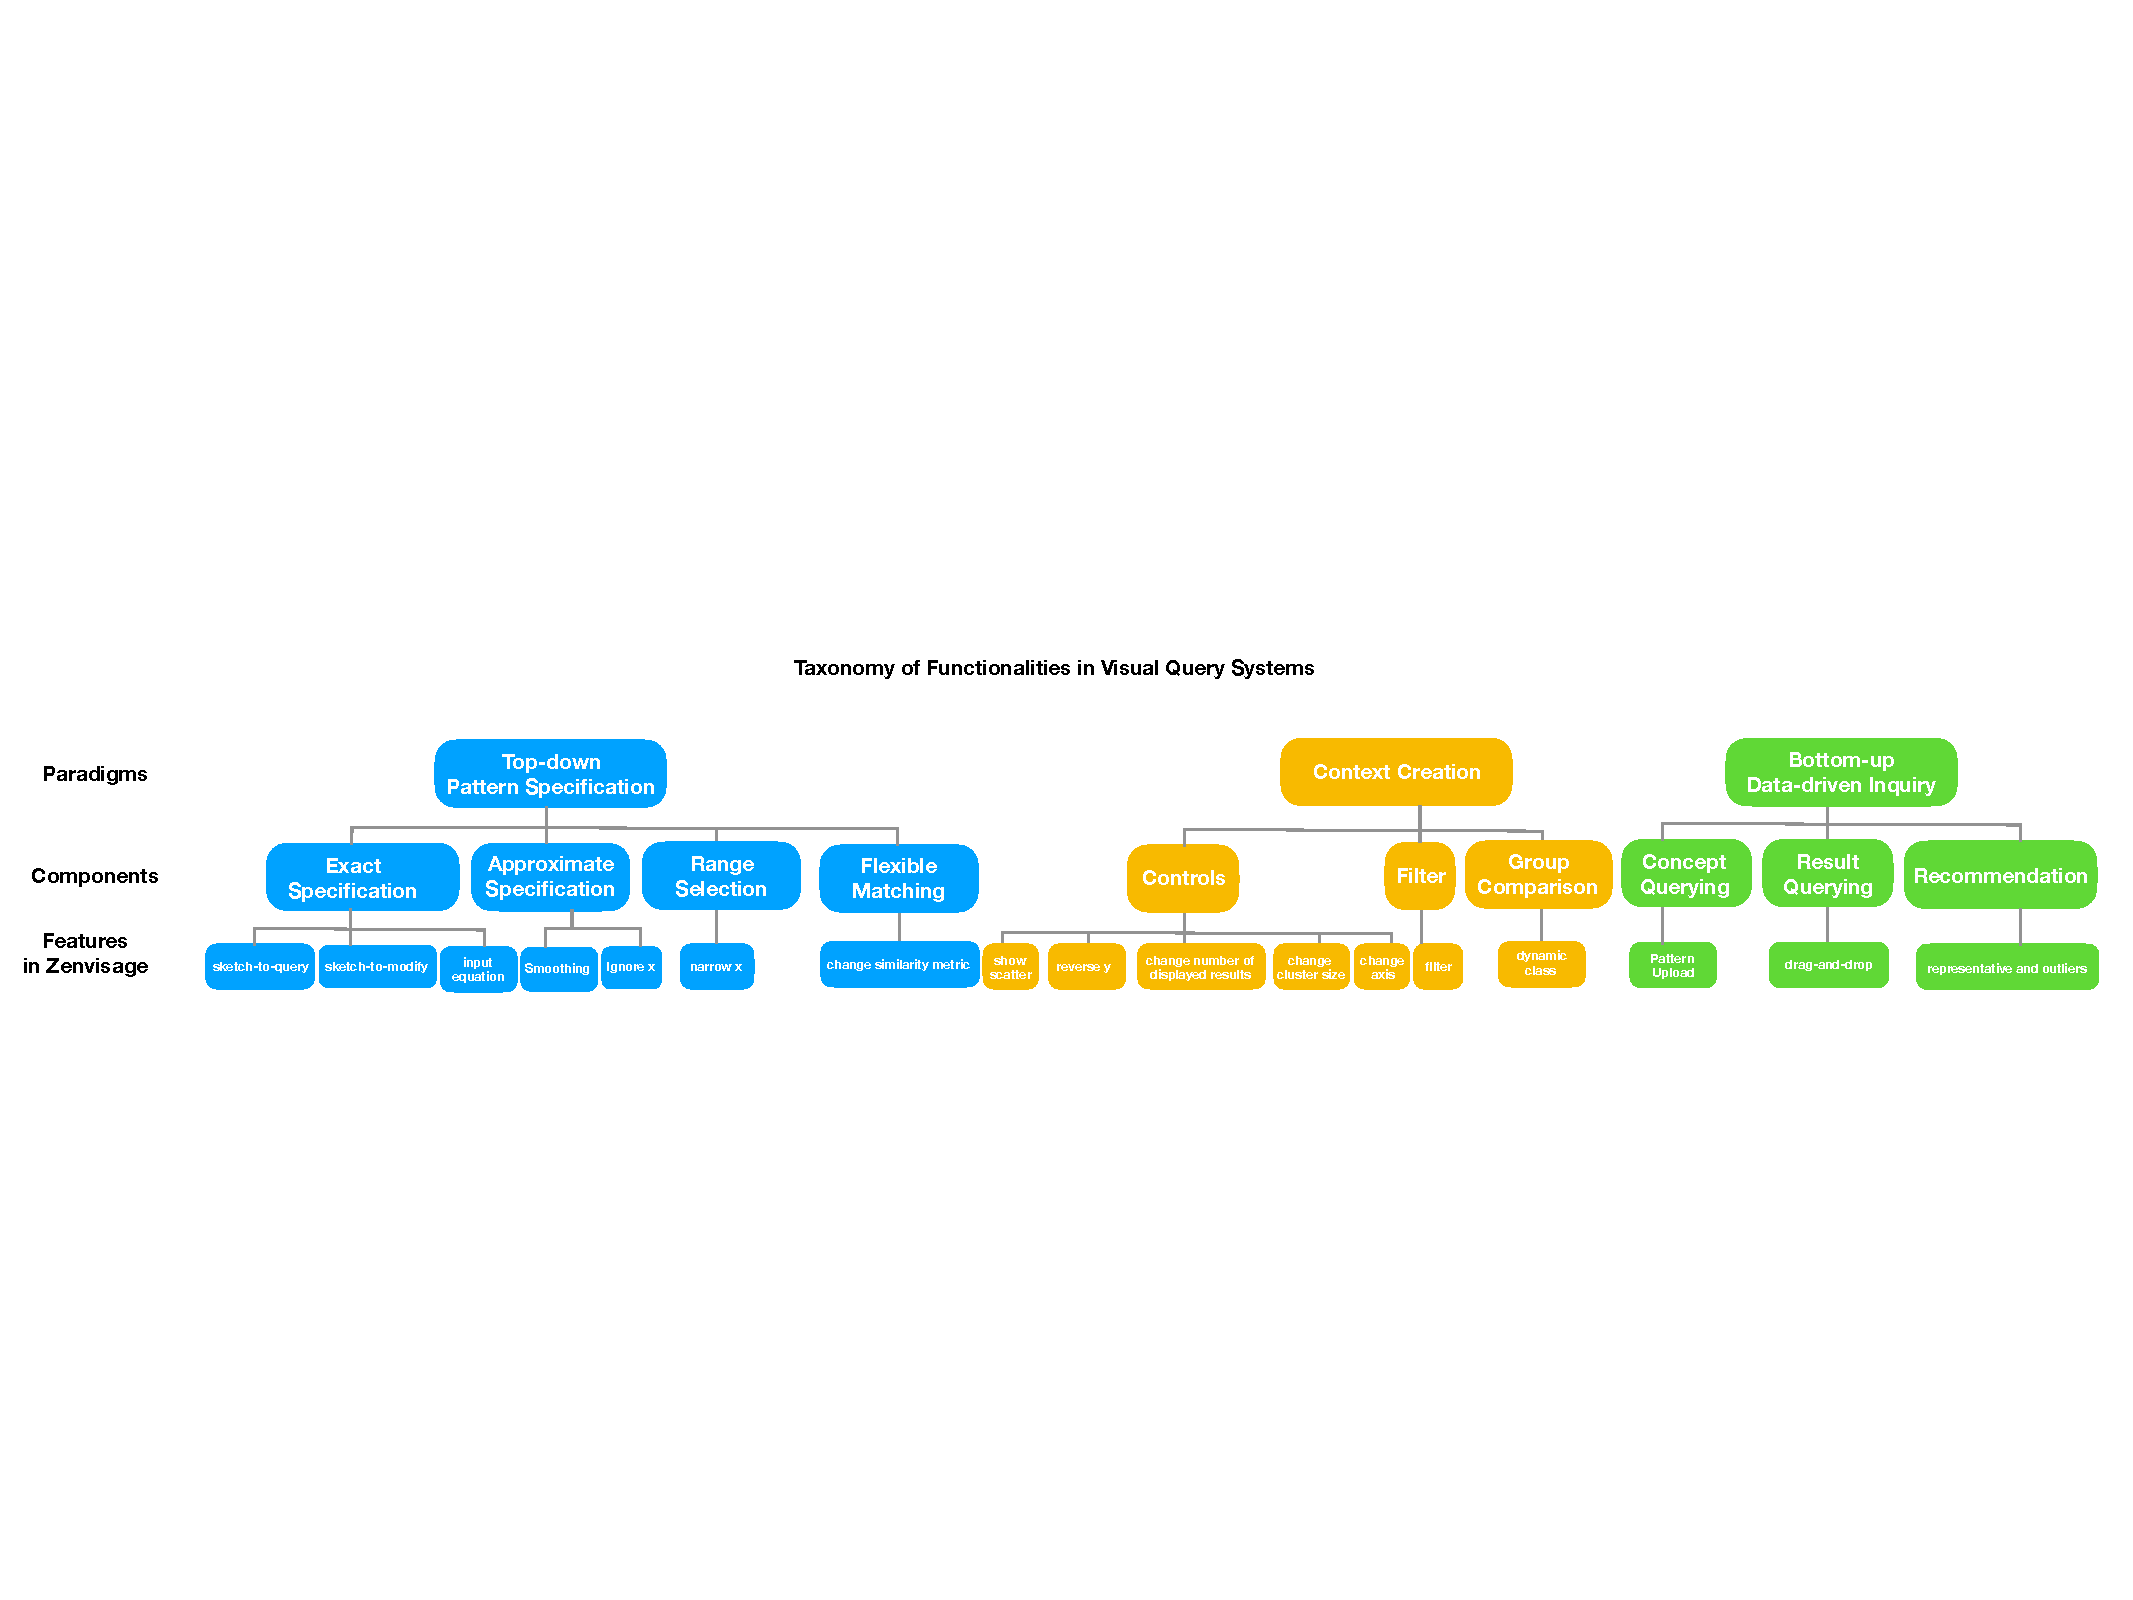
\includegraphics[width=\linewidth]{figures/taxonomy.pdf}
  \caption{Taxonomy of Functionalities in Visual Query Systems. From top, each of the three paradigm is broken down into key components in the system discussed in Section~\ref{pd_findings}, which is instantiated as features in \zv.}
  \label{fig:taxonomy}
\end{figure*}
Top-down Pattern Specification
- how to specify
- given known pattern, what is the amplitude, noise tolerance, etc. of a sketch? How to translate the in-the-head query to visual query and how matching is done
Bottom-up data-driven inquiry
- 
Context Creation
- 

\par While prior work has narrowed the focus of VQSs for use cases solely in the blue region, we envision opportunities for VQSs beyond this to a larger space of use cases and problems covered also by the red and green regions. We also note that the three processes that we have described are not mutually exclusive categories. In fact, we often see that participants construct a central workflow around one of the main paradigms and interleave variations with the two other processes as they iterate on the analytic task. 
\par Drawing from our participatory design experience, evaluation study, and literature review in this space, we describe the design challenge (DC) involved in building features that support these processes and how they tie in with characteristics of the analytic challenges presented by the use cases. In particular we motivate using evidence from how participants interact with the VQS during the evaluation study (e.g. analysis patterns, examples of real analysis insights). 
% \par As illustrated in Figure \ref{fig:sbmodel}, our search-browse paradigm is motivated by the characteristic challenges and foraging acts each use cases pose on existing VQSs observed in our design study. For example, the genetics participants do not have a preconceived knowledge of what they want to search for in the dataset. They were mostly interested in \textit{exploring} clusters to gain an overall sense what profiles exist in the dataset \tvcg{through representative trends} and therefore queried mainly through drag-and-drop to jumpstart further queries. Point to need for D3 and D4. The variations to their main workflow include changing cluster sizes and display settings to offer them different perspectives on the dataset (\textit{exploit}) and filtering on data attributes (\textit{enriching}).
% \par In the astronomy use case, the participants knew the patterns they are looking for, but the patterns are hard to specify and find. The main challenge for the VQS involves finer specification of sketched patterns, such as amplitude and width of the peak and noise level tolerance for defining a pattern match. Describe more in D1. The main workflow for the astronomers in our user study involves \textit{enriching}, either through finer query specification or via filtering data subsets, to increase the probability that their queries would be more accurately matched with what they are looking for.
% \par The main workflow for material scientists involves \textit{exploiting}, since they spend the majority of their efforts performing ``close-reading'' of individual visualizations to understand the relationships between physical variables. The participants are able to identify interesting relationships between physical variables when they examine each closely, but they are not sure what patterns to look for to begin with. More in D2.
% %For example, G2 knew that there was three repeated measurements that was taken for every timestep, in one of the profiles there was a sharp jump whereas other datapoints are relatively flat, he then concludes by inspecting in the scatterplot view that the rise in gene expression is probably due to an experimental error rather than the activation of a gene, because the other two repeated measurements were similar in magnitude. In other words, the scatterplot view offered him density of points as another proxy to consider that was not offered in the line chart perspective.
%  %This is true for both participants with and without a desired pattern in mind. For the participant without a desired pattern (G2), he created groups based on quartile statistics of additional data attributes and recorded the most significant representative pattern.

% - What does the act of browsing and searching mean in the context of VQSs
%   - browse: viewing ranked result and any recommended results on the side, derived from the data and analysis context.
%   - search: act of going from a user's in-the-head concept to an actionable query that could be executed through the VQSs, most work have focussed on sketch, we allow more than this.
%   - The challenge of browsing and searching is well-known in information retrieval~\cite{Olston2003}, browse alone is limited by how much a user can browse and process at once, search alone can be ambiguous without sufficient context from looking at example results.
% \par Pirolli and Card's notional model further characterizes the trade-offs between three central activities in the information foraging process: exploring, enriching, and exploiting~\cite{Pirolli}. \textit{Exploring} involves gathering more information during the analysis. \tvcg{In the context of VQSs}, exploring includes viewing representatives and outliers, incidental viewing of other visualizations \tvcg{in the ranked search results}, and querying via drag-and-drop and pattern-loading. \textit{Enriching} involves tasks that narrow down the space of analysis, such as filtering, dynamic class creation, query specification, and querying via input equations and sketching. \textit{Exploiting} involves spending time inspecting the results in more detail, including interpreting each visualization in greater detail or making plotting changes that offer another perspective (smoothing, display, and interpretability settings). We organize the features that we have developed in \zv into these foraging acts, as shown in Figure~\ref{feature_heatmap}.
% \par We find that participants often create unexpected workflows that chain together multiple analysis steps, including interactions, controls, and queries in order to address a higher-level research question. We find that participants often construct a central workflow, \tvcg{which they then iterate on while adding additional variations.} Their \emph{central workflow often resembles one of the three foraging acts} that aligns with the type of research question and dataset they are interested in. The variations are based on intermixing their central workflow with the other two foraging \tvcg{acts}.
% % We find that participants often have a strong inclination to perform tasks that resembles one of the three foraging act and sparsely intermixed with other activities to support their analysis, depending on the type of research question and dataset they are interested in.
% \par As illustrated in Figure \ref{fig:sbmodel}, our search-browse paradigm is motivated by the characteristic challenges and foraging acts each use cases pose on existing VQSs observed in our design study. For example, the genetics participants do not have a preconceived knowledge of what they want to search for in the dataset. They were mostly interested in \textit{exploring} clusters to gain an overall sense what profiles exist in the dataset \tvcg{through representative trends} and therefore queried mainly through drag-and-drop to jumpstart further queries. Point to need for D3 and D4. The variations to their main workflow include changing cluster sizes and display settings to offer them different perspectives on the dataset (\textit{exploit}) and filtering on data attributes (\textit{enriching}).
% \par In the astronomy use case, the participants knew the patterns they are looking for, but the patterns are hard to specify and find. The main challenge for the VQS involves finer specification of sketched patterns, such as amplitude and width of the peak and noise level tolerance for defining a pattern match. Describe more in D1. The main workflow for the astronomers in our user study involves \textit{enriching}, either through finer query specification or via filtering data subsets, to increase the probability that their queries would be more accurately matched with what they are looking for.
% \par The main workflow for material scientists involves \textit{exploiting}, since they spend the majority of their efforts performing ``close-reading'' of individual visualizations to understand the relationships between physical variables. The participants are able to identify interesting relationships between physical variables when they examine each closely, but they are not sure what patterns to look for to begin with. More in D2.
% %For example, G2 knew that there was three repeated measurements that was taken for every timestep, in one of the profiles there was a sharp jump whereas other datapoints are relatively flat, he then concludes by inspecting in the scatterplot view that the rise in gene expression is probably due to an experimental error rather than the activation of a gene, because the other two repeated measurements were similar in magnitude. In other words, the scatterplot view offered him density of points as another proxy to consider that was not offered in the line chart perspective.
%  %This is true for both participants with and without a desired pattern in mind. For the participant without a desired pattern (G2), he created groups based on quartile statistics of additional data attributes and recorded the most significant representative pattern.
% % [---] out of 9 of our participants had more than one main workflow.

\subsection{DP1: The Inefficiency of Sketch}
% \subsection{DC3: Closing the loop in VQS sense-making cycle with bottom-up data-driven inquries}
\par In the context of visual querying, top-down approaches are query specification methods based on users' preconceived notion of what to search for. As shown in Figure~\ref{taxonomy}, this includes both components for specifying the pattern as well as controls governing the underlying algorithm of how the shape-matching is performed. Our interactions with the scientists showed that different modalities for inputting a query can be useful for different problem contexts.
\par To our surprise, despite the prevalence of sketch-to-query systems in literature, only two out of our nine users had a practical usage for querying by sketching. Overall, bottom-up querying via drag-and-drop was more intuitive and more commonly used than top-down querying methods, such as sketching or input equations.
\par The main reason why participants did not find sketching useful was that they often do not start their analysis with a pattern in mind. Later, their intuition about what to query is derived from other visualizations that they see in the VQS, in which case it made more sense to query using those visualizations as examples directly (via drag-and-drop). In addition, even if a user has a query pattern in mind, sketch queries can be ambiguous or impossible to draw by sketching (e.g. A2 looked for a highly-varying signal enveloped by a sinusoidal pattern indicating planetary rotation).
\par Likewise, despite functional fitting being common in scientific data analysis, Figure \ref{feature_heatmap} shows that querying by equation is also unpopular for similar reasons. In addition, the visualizations for both astronomy and genetics exhibit complex processes that could not be written down as an equation analytically. However, even when analytical relationships do exist (in the case of material science), it is challenging to formulate functional forms in an prescriptive, ad-hoc manner. 
\par The latter case is also evident from the unexpected use cases where sketching was simply used as a mechanism to modify dragged-and-dropped queries. As shown in Figure \ref{query_modification} (top), M2 first sketched a pattern to find solvent classes with anticorrelated properties. However, the sketched query did not return the visualization he was interested in. So, he instead dragged and dropped one of the peripheral visualizations that was close enough to his desired visualization to the sketchpad and then smoothed out the noise due to outlier datapoints by tracing a sketch over the visualization. M2 repeated this workflow twice in separate occurrences during the study and was able to derive insights from the results. Likewise, A3 was interested in pulsating stars characterized by dramatic changes in the amplitudes of the light curves. During the search, hotspots on stellar surfaces often show up as false positives as they also result in dramatic amplitude fluctuations, but happen at a regular intervals. In the VQS, A3 looked for patterns that exhibits amplitude variations, but also some irregularities. As shown in Figure \ref{query_modification} (bottom), she first picked out a regular pattern (suspected star spot), then modified it slightly so that the pattern looks more irregular.
\begin{figure}[ht!]
    \centering
    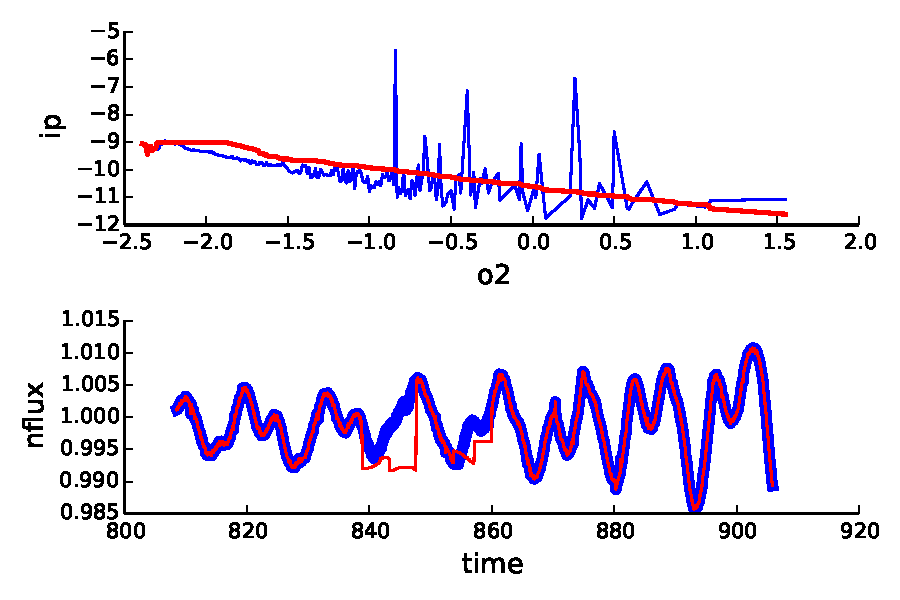
\includegraphics[width=\columnwidth]{figures/QueryModificationBySketch.pdf}
    \caption{\tvcg{Examples of query modification by M2 (top) and A3 (bottom) performed during the study The inital drag-and-dropped query is shown in blue and the sketch-modified queries in red.}
    \label{query_modification}}
    \vspace{-10pt}
\end{figure}
\par Both of these use cases suggest that while sketching is an useful analogy for people to express their queries, \emph{the existing ad-hoc, sketch-only model for visualization querying is insufficient without data examples that can help analysts jumpstart their exploration}. Table~\ref{table:relatedwork} also show that most past work focus on optimizing the components in the top-down paradigm, missing out largely on the key components in the other two paradigms, indicated by the absence of green features on the right hand side of the table. We suspect that the limited coverage in addressing different types of analytics use cases may be why existing sketch-to-query systems are not commonly adopted in practice. %This result points to a need for ----- in future VQSs. %This, however, points to an exciting direction for sketching interface in VQSs for developing advanced drawing and modification tools that enable more precise visualization query specification.}
%For instance, material science discovered a known inverse relationship during exploration
%Which is really interesting. Which is something that we observed experimentally also. That is an interesting insight right htere. This seems to suggest that there is a fundamental issue in if you want to try to get better on this axis, and get as low as possible, you lose out on the other axis.
%once they see it they know it but they don't know beforehand

\subsection{DP2: Usefulness of bottom-up approaches}
\par While the usage of each querying feature may vary from one participant to the next, generally, result querying and pattern upload are considered bottom-up approaches that go from data to theory by enabling users to query via examples of known visualizations. For top-down approaches such as query by sketching and input equations, the user starts with an intuition about how their desired patterns should look like based on theory, then queries based on that. Our results indicate that \emph{bottom-up querying approaches are preferred over top-down when the users have no desired patterns in mind}, which is commonly the case for exploratory data analysis.
\par Examples of practical uses of result querying includes inspecting the top-most similar visualizations that lie in a cluster and finding visualizations that are similar to an object of interest that exhibits a desired pattern. Likewise, many participants envisioned use cases for pattern loading. The ability to load in data patterns as a query would enable users to compare visualizations between different experiments, species, or surveys, query with known patterns from an external reference catalog (e.g. important genes of interest, objects labeled as supernovae), or verify the results of a simulation or downstream analysis by finding similar patterns in their existing dataset. In addition, users can also specify a more precise query that captures the essential shape features of a desired pattern (e.g. amplitude, width of peak), that  cannot be precisely drawn as a sketched pattern. For example, Figure \ref{example} (left) shows that the width of the light curve is characteristic to the type of supernovae that it is associated with, so querying with an exact pattern template would be helpful for distinguishing the patterns of interest from noise.
\par The prevalence of bottom-up approaches not only point to the need for supporting result querying in VQSs, but it also points to the need for providing recommendation for users who may not have a desired pattern in mind. We found that geneticists often gain their intuition about the data from the recommended representative trends. One example of rapid insight discovery comes from G2, and G3, who identified that the three representative patterns shown in \zv---induced genes (profiles with expression levels staying up), repressed genes (started high but went down), and transients (go up and then come down at different time points)---corresponded to the same three groups of genes discussed in a recent publication\cite{Gloss2017}.
\par The clusters provoked G2 to generate a hypothesis regarding the properties of transients: \textit{``Is that because all the transient groups get clustered together, can I get sharp patterns that rise and ebb at different time points?''} To verify this hypothesis, G2 increased the parameter controlling the number of clusters and noticed that the cluster no longer exhibited the clean, intuitive patterns he had seen earlier. G3 expressed a similar sentiment and attempted to identify different clusters. He proceeded by inspecting the visualizations in the cluster via drag-and-drop and found a group of genes that all transitioned at the same timestep, while others transitioned at different timesteps. G3 described the process of using VQSs as doing ``detective work'' that provoked him to generate further scientific hypotheses as well as data actions.
\par By browsing through the ranked list of result, representative, and outlier in \zv, participants were also able to gain a peripheral overview of the data and spot anomalies during exploration. For example, A1 spotted time series that were too faint to look like stars after applying a filter constraint of CLASS\_STAR=1. After a series of query results browsing and consultation with an external database, he concluded that the dataset had been incorrectly labelled with all the stars with CLASS\_STAR=0 as 1 during data cleaning. These examples show that both the browsing-act through recommendations and performing search via these results are essential for `closing the loop' between the sensemaking loop in VQSs. 
\subsection{DP3: Enriching Search with Context}
\par Past studies in taxonomies of visualization tasks have shown that it is important to design features that enable users to select relevant subsets of data in visual analytics\cite{Amar2005,Heer2012}. %We designed two dynamic faceting features coupled with coordinated views that enabled users to specify subsets of data they are querying on and see immediate changes updated in the query, representative, and outlier results.
We found that all participants either envisioned a use case or utilized components of the context creation paradigm offered in \zv to explore and compare subsets of their data.
\par A1 expressed that even though the filtering step could be easily done programmatically on the dataset and reloaded into \zv, filtering on-the-fly was a powerful way to dynamically test his hypothesis. Interactive filtering lowers the barrier between the iterative hypothesize-then-compare cycle, thereby enabling participants to test conditions and tune values that they would not have otherwise modified as much.
% echoing our previous finding that segmented workflow prevents extensive exploration.
During the study, participants used filtering to address questions such as: \textit{Are there more genes similar to a known activator when we subselect only the differentially expressed genes?} \texttt{DIFFEXP=1} (G2) or \textit{Can I find more supernovae candidates if I query only on objects that are bright and classified as a star?} \texttt{flux\textgreater10 AND CLASS\_STAR=1} (A1). Three participants had also used filtering as a way to pick out individual objects of interest to query with. For example, G2 set the filter as gene=9687 and explained that since ``this gene is regulated by the estrogen receptor, when we search for other genes that resemble this gene, we can find other genes that are potentially affected by the same factors.''
As shown in Figures \ref{action_heatmap} and \ref{feature_heatmap}, participants with the top-most provoked data actions (A1, A3, G2) made heavy use of filtering to explore different subsets of the data.
\par While filtering enabled users to narrow down to a selected data subset, dynamic class creation enabled users to compare relationships between multiple attributes and between subgroups of data. For example, M2 divided solvents in the database to eight different categories based on voltage properties, state of matter, and viscosity levels, by dynamically setting the cutoff values on the quantitative variables to create these classes. By exploring these custom classes, M2 learned that the relationship between viscosity and lithium solvation energy is independent of whether a solvent belongs to the class of high voltage or low voltage solvents and cited that dynamic class creation was central to learning about this previously-unknown attribute properties:
\begin{quote}
All this is really possible because of dynamic class creation, so this allows you to bucket your intuition and put that together. [...] I can now bucket things as high voltage stable, liquid stable, viscous, or not viscous and start doing this classification quickly and start to explore trends. [...] And look how quickly we can do it! Quite good!
\end{quote}
%Context creation is a useful ---- despite the --- pattern instance. Filtering still useful 
%\par Participants employed \emph{a mix of bottom-up and top-down approaches when faceting through data in VQS}, including narrowing the search space based on some intuition about a phenomena, selecting individual visualizations, or specifying high-level groupings to compare and query with.